

\documentclass[../../e3_tp2_main.tex]{subfiles}

\begin{document}
\section{Ejercicio 7}


Se implementaron un contador sincrónico y otro asincrónico con compuertas lógicas. Se compararon sus funcionamientos y se halló la máxima velocidad de operación de cada uno.

\subsection{Contador sincr\'onico}
Los contadores sincrónicos son aquellos en los cuales todos sus flip flop cambian de estado al mismo tiempo. Esto se debe a que cada flip clop comparte el mismo \textit{clock}.
\subsubsection{Funcionamiento}
Tal como se mencionó anteriormente, un contador asincrónico basa su funcionamiento en flip flops, particularmente de tipo T.
\par El circuito lógico correspondiente al contador sincrónico de 3 bits es el siguiente:


\begin{figure}[H]	
	\centering
	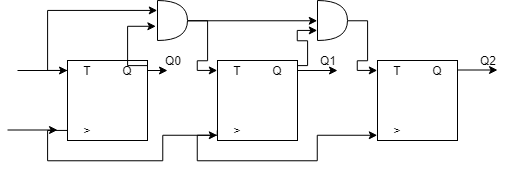
\includegraphics[width=0.45\textwidth]{imagenes/cs_b.png}
	\caption{Circuito digital contador sincr\'onico}\label{fig:cse}
\end{figure}
Este contador es sincrónico de tres bits ascendente (desde cero), donde Q0, Q1 y Q2 son las salidas del contador. La entrada del circuito es un pin de \textit{enable} y otro de \textit{clock}.

\subsubsection{Implementación y Medicion}

Se implementó el circuito previamente mencionado con compuertas \textit{and} (74HC00) y flip flops SR (CD4027). Juntando los terminales del SR se obtuvo el flip flop T.
\par En la siguiente imagen se observa el funcionamiento del contador:

\begin{figure}[H]	
	\centering
	\fbox{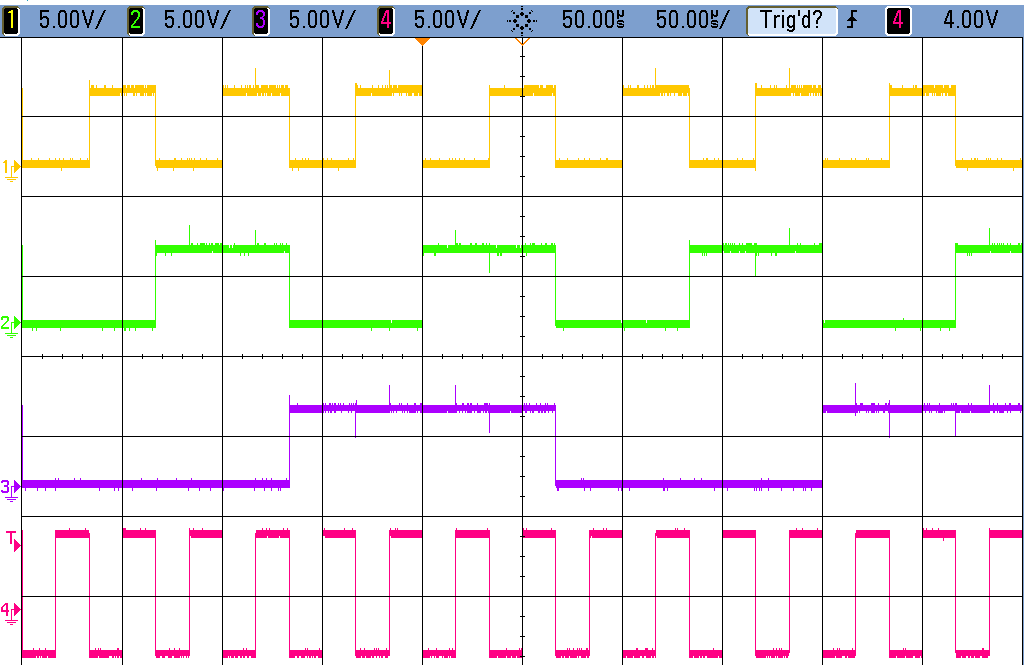
\includegraphics[width=0.45\textwidth]{imagenes/cs_count.png}}
	\caption{Funcionamiento del contador (\textit{clock} en rosa, Q0 amarillo, Q1 verde, Q2 violeta)}
\end{figure}

\begin{figure}[H]	
	\centering
	\fbox{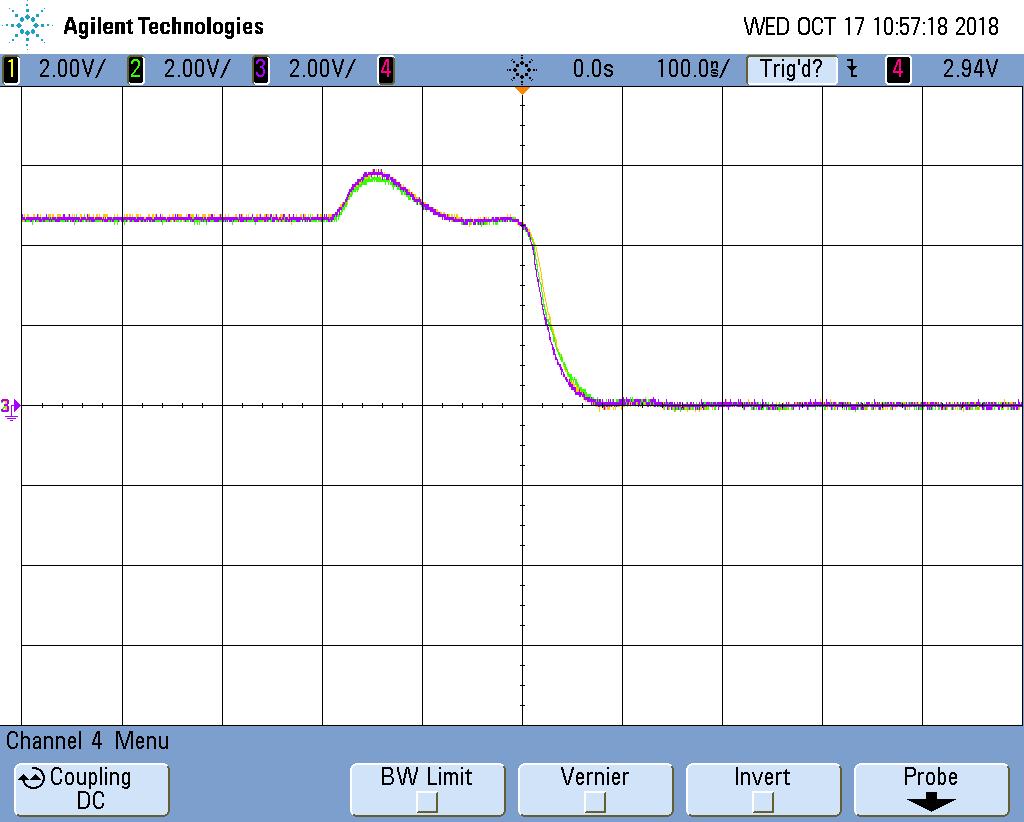
\includegraphics[width=0.45\textwidth]{imagenes/cs_f.png}}
	\caption{Contador pasando de 7 a 0 (\textit{clock} en rosa, Q0 amarillo, Q1 verde, Q2 violeta)} \label{fig:s1t0}
\end{figure}

En la figura \ref{fig:s1t0} se observa c\'omo el cambio se estado en los tres flip flops ocurre de forma pr\'acticamente instant\'anea.

\subsubsection{Máxima velocidad de conteo}
La máxima velocidad a la que puede contar el circuito propuesto, depende de tres factores: el tiempo de establecimiento del flip flop, el de la compuerta \textit{and}, y el tiempo de \textit{set up} (es decir, el que se requiere para que el sistema se estabilice).
\par De esta manera queda definida la máxima frecuencia del clock:
$$f_{C_{MAX}}=\frac{1}{t_{e_{AND}} +t_{e_{Flipflop}} +t_{setup}   } $$

\subsection{Contador asincr\'onico}
Los contadores asincrónicos son aquellos en los cuales la señal de \textit{clock} ingresa por uno de los flip flops y se propaga por el resto.

\subsubsection{Funcionamiento}

El contador asincrónico basa su funcionamiento en flip flops T. A diferencia del contador sincr\'onico, los flip flpos no comparten \textit{clock}, sino que se conectan en cascada. 
\par El circuito lógico correspondiente es el siguiente:


\begin{figure}[H]	
	\centering
	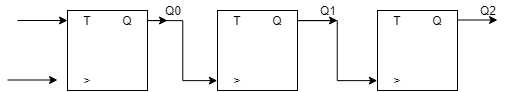
\includegraphics[width=0.45\textwidth]{imagenes/cas_b.png}
	\caption{Circuito digital contador asincr\'onico}\label{fig:case}
\end{figure}

Este contador es asincr\'onico de tres bits ascendente (desde cero), donde Q0 a Q2 son las salidas del contador. La entrada del circuito es un pin de \textit{enable} y otro de \textit{clock}.

\subsubsection{Implementación}
Se implementó el circuito anteriormente indicado, con flip flops SR (CD4027). Juntando los terminales del SR se obtuvo un flip flop T.

\par En la siguiente imagen se observa el funcionamiento del contador:

\begin{figure}[H]	
	\centering
	\fbox{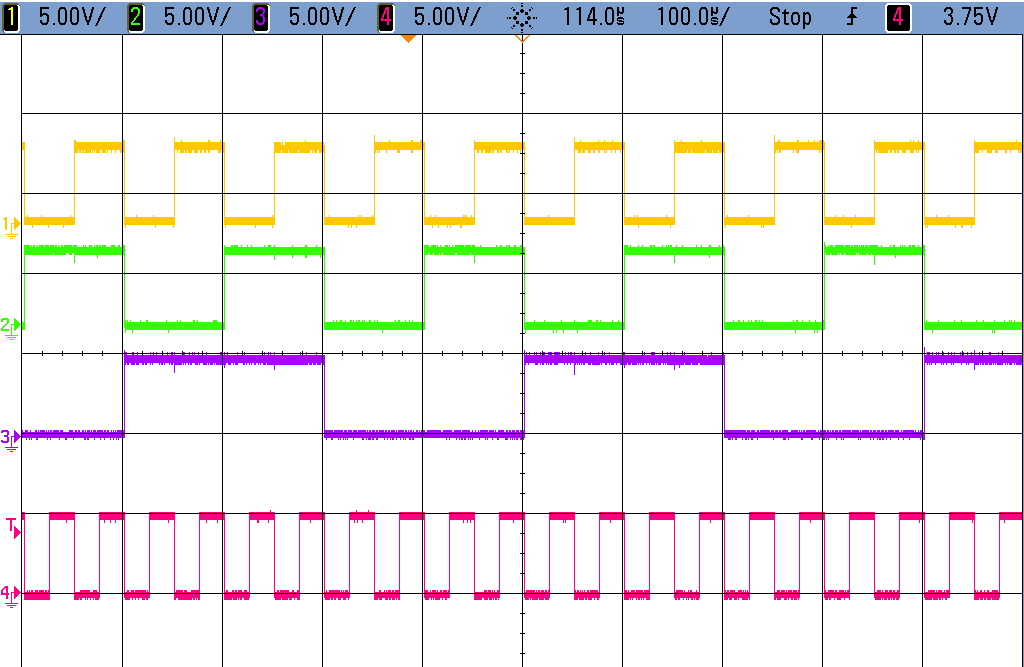
\includegraphics[width=0.45\textwidth]{imagenes/cas_count.png}}
	\caption{Funcionamiento del contador (\textit{clock} en rosa, Q0 amarillo, Q1 verde y Q2 violeta)}
\end{figure}

\begin{figure}[H]	
	\centering
	\fbox{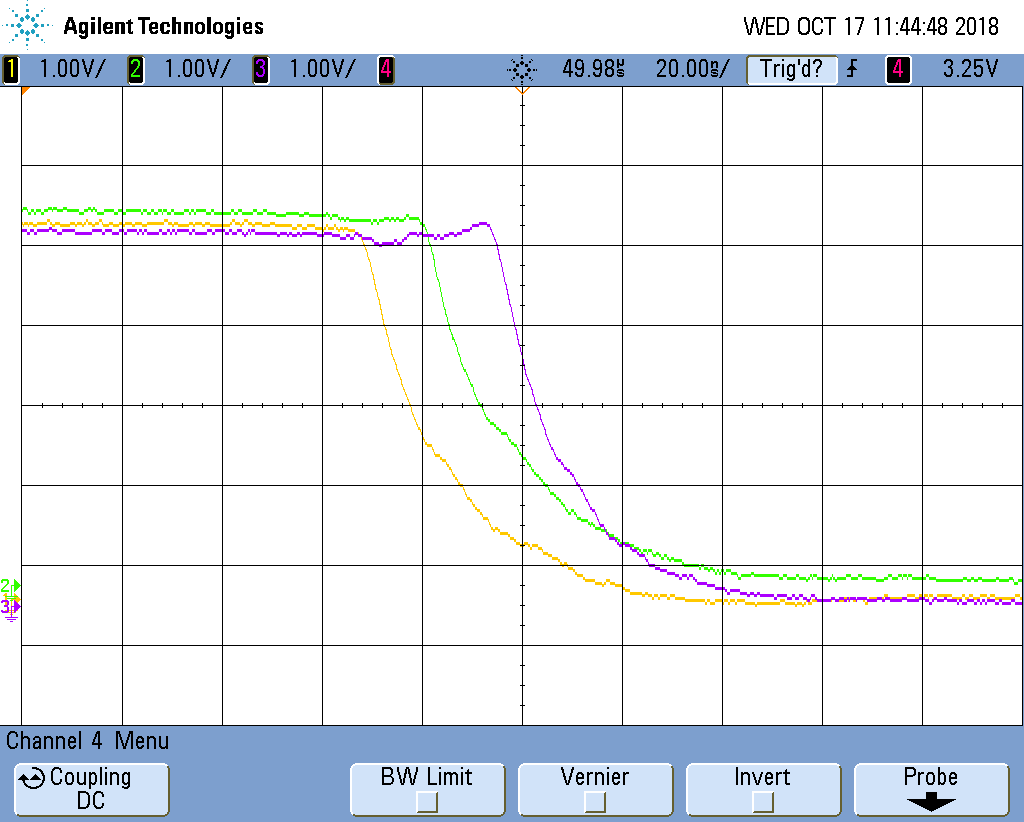
\includegraphics[width=0.45\textwidth]{imagenes/cas_f.png}}
	\caption{Contador pasando de 7 a cero (\textit{clock} en rosa, Q0 amarillo, Q1 verde y Q2 violeta)} \label{fig:as1t0}
\end{figure}

En la figura \ref{fig:as1t0} se observa que los tiempos entre cada salida son mayores que los que se obtuvieron para el contador sincr\'oinco, lo cual era lo esperado dado que que el \textit{clock} se debe propagar por cada flip flop.

\subsubsection{Máxima velocidad de conteo}
A diferencia del contador sincrónico, en el asincrónico la velocidad máxima de operación depende del tiempo de establecimiento de cada flip flop. Por ende la máxima frecuencia de clock soportada es la siguiente (donde N es el n\'umero de flip flops utilizados):
$$f_{c_{MAX}}=\frac{1}{N \cdot t_{e_{Flipflop}}} $$


\end{document}
